% !TEX root = domain_transduction.tex
We evaluate our algorithm on various unsupervised domain adaptation tasks while focusing on two different problems, hand-written digit classification and object recognition. For each experiment, we use three domains and evaluate all adaptation scenarios.

\begin{table*}[ht]
\setlength{\tabcolsep}{3pt}
\vspace{-3mm}
\caption{Accuracy of our method and the state-of-the-art algorithms on Office dataset and various adaptation settings}
\label{tab:res}
\begin{sc}
\begin{center}
\begin{small}
\resizebox{\columnwidth}{!}{%
\begin{tabular}{@{}rcccccc@{}} \toprule 
 Source & Amazon & D-SLR & Webcam & Webcam &Amazon & D-SLR \\
 Target & Webcam & Webcam & D-SLR & Amazon & D-SLR & Amazon \\
 \midrule
GFK \cite{gong2012} & $.398$ & $.791$ & $.746 $ & $.371$ & $.379$ & .379   \\
SA* \cite{fernando13} & $.450$ & $.648$ & $.699$ & $.393$ & $.388$ & $.420$ \\
DLID \cite{chopra13} & $.519$ & $.782$ & $.899$ & -&- &- \\
DDC \cite{tzeng14} & $.618$ & $.950$ & $.985$ & $.522$ & $.644$& $.521$\\
DAN \cite{wang15} & $.685$ & $.960$ & $.990$ & $.531$ & $.670$ & $.540$ \\
Backprop \cite{ganin15} & $.730$ &$.964$ & $.992$ & $.536$ & $.728$ & $.544$\\
\midrule
Source Only & $.642$ & $.961$ & $.978$ & $.452$ & $.668$ & $.476$ \\
Our Method (no reject/no prop) & $.727$ &.952 & $.915$ & $.575$ & $.791$ & $.521$ \\
Our Method (no reject) & $.804$ &$.962$ & $.989$ & $.625$ & $.839$ & $.567$ \\
Our Method (full) & $\mathbf{.814}$ & $\mathbf{.971}$ & $\mathbf{.993}$ & $\mathbf{.663}$ & $\mathbf{.847}$ & $\mathbf{.601}$ \\
\bottomrule
\end{tabular}}
\end{small}
\end{center}
\end{sc}
\vspace{-5mm}
\end{table*}

\subsection{Dataset}
We use MNIST~\cite{mnist}, Street View House Number~\cite{svhn} and the artificially generated version of MNIST -MNIST-M-~\cite{ganin15} to experiment our algorithm on the digit classification task. MNIST-M is simply a blend of the digit images of the original MNIST dataset and the color images of BSDS500~\cite{bsds500} following the method explained in \cite{ganin15}. Since the dataset is not distributed directly by the authors, we generated the dataset using the same procedure and further confirmed that the performance is the same as the one reported in \cite{ganin15}. Street View House Numbers dataset is a collection of house numbers collected directly from Google street view images. Each of these three domains are quite different from each other and among many important differences, the most significant ones are MNIST being grayscale and the others being colored, and SVHN images having extra confusing digits around the centered digit of interest. Moreover, all three domains are large-scale having at least 60k examples over 10 classes. 

\begin{wraptable}{r}{0.5\textwidth}
%\begin{table}[ht]
\setlength{\tabcolsep}{3pt}
\caption{Accuracy on the digit classification task.}
\label{tab:res2}
\begin{sc}
\begin{small}
\resizebox{0.5\textwidth}{!}{%
\begin{tabular}{@{}r@{\hskip 1mm}c@{\hskip 1mm}c@{\hskip 1mm}c@{\hskip 1mm}c@{}} \toprule 
Source & M-M & MNIST  & SVHN & MNIST \\
Target&  MNIST & M-M & MNIST & SVHN\\
 \midrule
SA* \cite{fernando13}& $.523$ & $.569$ & $.593$ & $.211$ \\
BP \cite{ganin15} &$.732$ & $.766$ & $.738$ & $.289$ \\
\midrule
Source Only  & $.483$ & $.522$  &.549 & $.162$  \\
Our Method & $\mathbf{.835}$ & $\mathbf{.855}$ & $\mathbf{.774}$ & $\mathbf{.323}$\\
 \bottomrule
\end{tabular}}
\end{small}
\end{sc}
\end{wraptable}

In addition, we use the Office~\cite{office} dataset to evaluate our algorithm on the object recognition task. Office dataset includes images of the objects taken from Amazon, captured with a webcam and captured with a D-SLR. Differences between domains include the white background of Amazon images vs realistic webcam images, and the resolution differences. The Office dataset has fewer images, with a maximum of 2478 per domain over 31 classes. %On the other hand, it has larger number of classes over 31 categories.

\subsection{Baselines}
We compare our method with a variety of methods with and without feature learning. Considering the two different lines of work, \textbf{SA*}\cite{fernando13} is the dominant state-of-the-art approach not employing any feature learning, and \textbf{Backprop(BP)}\cite{ganin15} is the dominant state-of-the-art employing feature learning. We use the available source code of \cite{ganin15} and \cite{fernando13} and following the evaluation procedure in \cite{ganin15}, we choose the hyper-parameter of \cite{fernando13} as the highest performing one among various alternatives. We also compare our method with the \textbf{source only} baseline which is a convolutional neural network trained only using the source data. This classifier is clearly different from our nearest neighbor classifier; however, we experimentally validated that CNN always outperformed the nearest neighbor based classifier. Hence, we report the highest performing source only method.

\subsection{Implementation Details}
\label{imp_det}
Although our algorithm has very few hyper-parameters and we choose most of them either using cross-validation or exhaustive grid search, our algorithm uses an existing differentiable feature function. Following the unparalleled success of convolutional neural networks (CNNs), we use CNNs as our feature functions.  We consider the last fully connected layer as domain specific feature ($\theta_s$, $\theta_t$) and the rest as common network $\theta_c$. Common network weights are tied between domains. In order to have a fair comparison with existing algorithms, we follow the same architecture used by \cite{ganin15} by only changing the final feature dimensionality (embedding size). We use the following architectures for domains:

\noindent \textbf{MNIST} and \textbf{SVHN:} LeNet\cite{lenet} as; 
\includegraphics[width=0.5\columnwidth]{lenet}

\noindent \textbf{Office:} AlexNet\cite{alexnet} as; 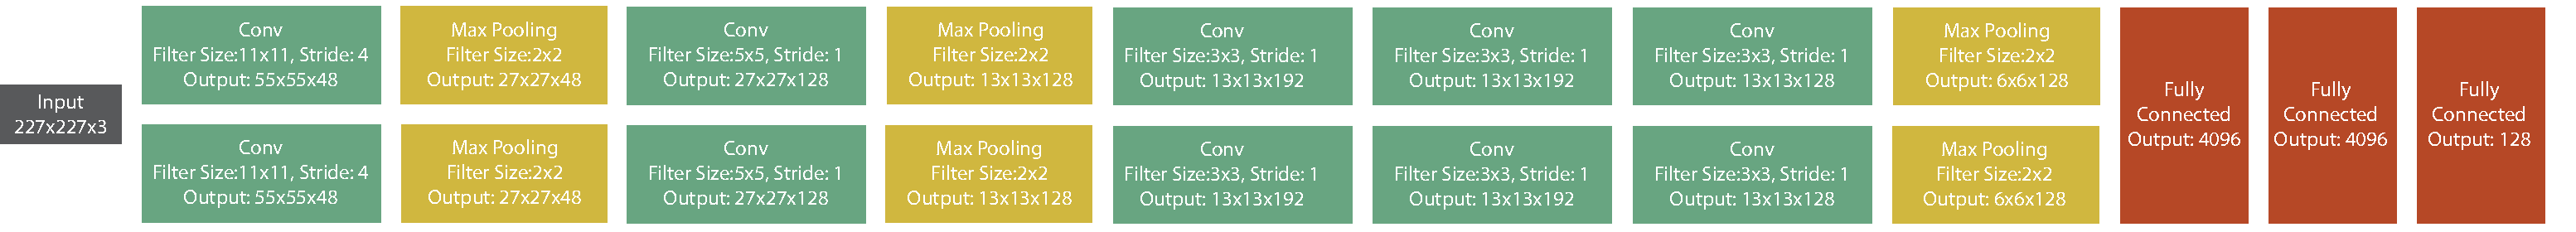
\includegraphics[width=0.55\columnwidth]{alexnet}

where \textbf{C} is convolution, \textbf{P} is max-pooling, \textbf{R} is ReLU and \textbf{F} is fully connected layer. 

Since the office dataset is quite small, we do not learn the full network for office experiments and instead we only optimize for fully connected layers initializing with the weights pre-trained on ImageNet. In all of our experiments, we set the feature dimension as $128$. We use stochastic gradient descent to learn the feature function with AdaGrad\cite{adagrad}. We initialize variables with truncated normals having unit variance and use the learning rate \SI{2.5e-4}  and the batch size $256$. We start the rejection penalty with $\gamma=0.5$ and linearly increases with each epoch as $\gamma=\frac{epoch\quad cnt}{20}$.

\subsection{Evaluation Procedure}
We evaluate all algorithms in fully transductive setup following the standard evaluation setup of \cite{office}.  We feed training images and labels of the first domain as the source and training images of the second domain as the target. We further evaluate the accuracy on the target domain labels as the ratio of correctly labeled images to all target images.

\subsection{Results}
Following the fully transductive evaluation, we summarize the results in Table~\ref{tab:res} and Table~\ref{tab:res2}. Table~\ref{tab:res} summarizes the results on the object recognition task using office dataset whereas  Table~\ref{tab:res2} summarizes the digit classification task on MNIST and SVHN.

Table~\ref{tab:res}\&\ref{tab:res2} shows results on object recognition and digit classification tasks exhaustively covering all adaptation scenarios. Our algorithm shows state-of-the-art performance. Moreover, our algorithm significantly outperforms all state-of-the-art methods when there is a large domain difference such as MNIST$\leftrightarrow$MNIST-M, MNIST$\leftrightarrow$SVHN, Amazon$\leftrightarrow$Webcam and Amazon$\leftrightarrow$D-SLR. Our hypothesis is that the state-of-the-art algorithms like \cite{ganin15} are seeking for set of features invariant to the domains whereas we seek for an explicit similarity metric explaining both differences and similarities of domains. In other words, instead of seeking for an invariance, we seek for an equivariance.

\iffalse
\begin{wrapfigure}{r}{0.5\textwidth}
\vspace{-1mm}
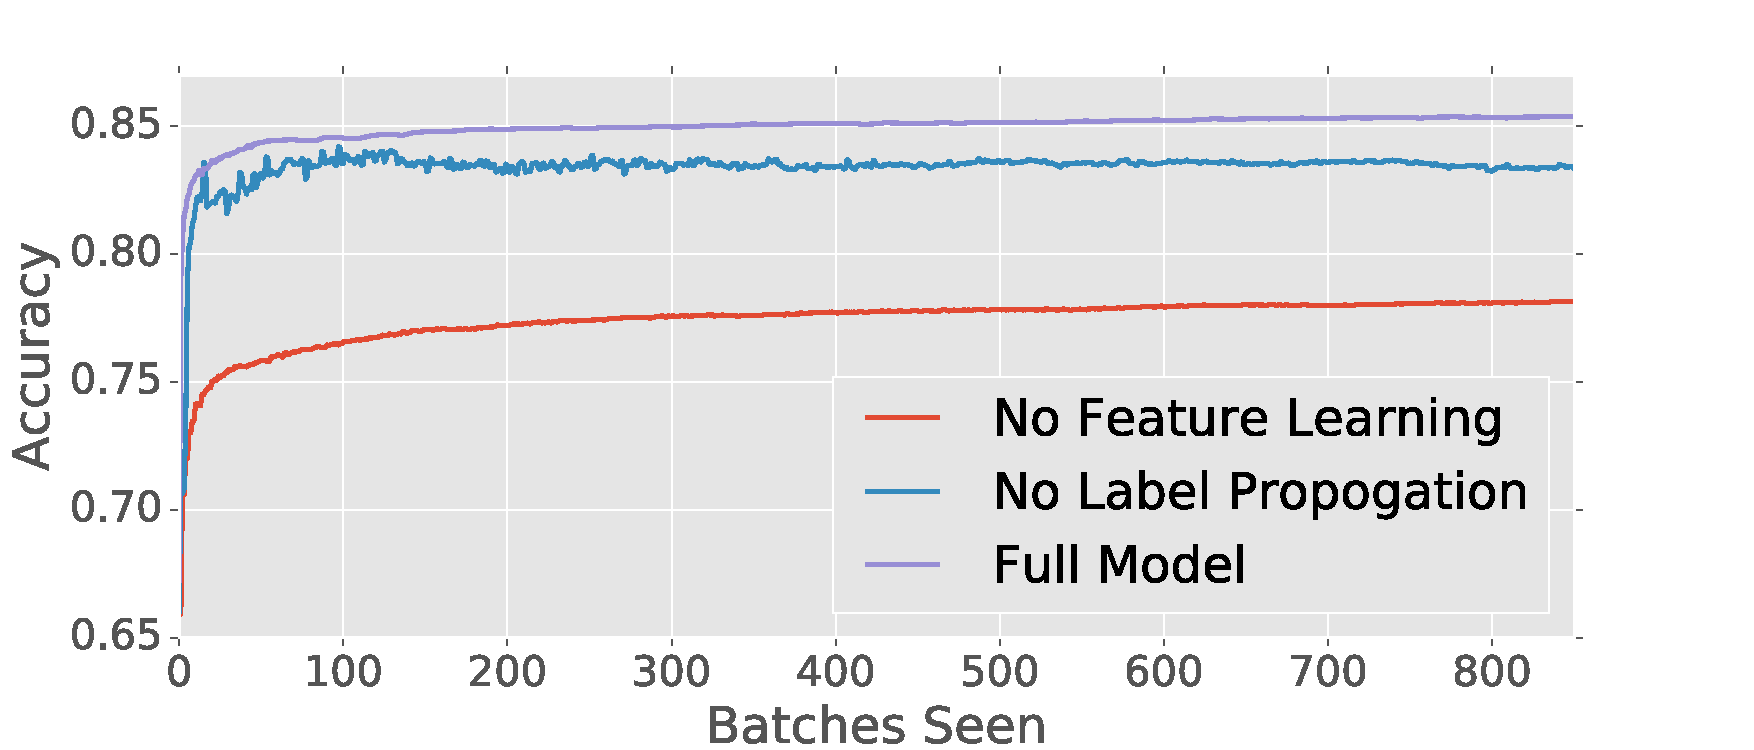
\includegraphics[width=0.5\textwidth]{no_feature_propogation}
\vspace{-6mm}
\caption{Accuracy vs number of iterations for our method and its variant without label propagation as well as the variant without feature learning. As the figure suggests the label propagation increases both the stability of the gradients as well as the final accuracy. Moreover, the feature learning also has a significant effect on the accuracy.}
\label{fllprop}
\end{wrapfigure}
\fi

Table~\ref{tab:res2} further suggests our algorithm is the only one which can generalize that well from MNIST to SVHN dataset. Clearly the features which are learned from MNIST cannot generalize to SVHN since the SVHN has concepts like color and occlusion which are not available in MNIST. Hence, our algorithm learns SVHN specific features by enforcing accurate transduction in the adaptation stage.

Another interesting conclusion is the asymmetric nature of the results. For example, the accuracy of adapting webcam to amazon and adapting Amazon to webcam is significantly different in Table~\ref{tab:res}. The similar behavior exists in MNIST and SVHN domains as well in Table~\ref{tab:res}. This observation validates the importance of an asymmetric modeling.

\subsubsection{Qualitative Analysis}
To further study the learned representations as well as the similarity metric, we perform a series of qualitative analysis in the form of nearest neighbor analyses and tSNE\cite{tsne} plots.

Figure~\ref{fig:nn} visualizes example target images from MNIST and their corresponding source images. First of all, both our experimental procedure and qualitative analysis suggest that MNIST and SVHN are the two domains with the largest difference. Hence, we believe MNIST$\leftrightarrow$SVHN is very challenging set-up and despite the huge visual differences, our algorithm results in accurate nearest neighbors.

Figure~\ref{fig:nnoffice} visualizes the example target images from webcam and their corresponding nearest source images from Amazon. The difference between invariance and equivariance is more clear in the tSNE plots of the Office dataset in Figure~\ref{fig:tsne} as well as digit classification task Figure~\ref{fig:tsnedigit}. In Figure~\ref{fig:tsne}, we plot the distribution of features before and after adaptation for source and target while color coding class labels. As Figure~\ref{fig:tsne} suggests, the source domain is well clustered according to the object classes with and without adaptation. Moreover, this is expected since the features are specifically fine-tuned to the source domain before the adaptation starts. However, target domain features have no structure before adaptation. This is also expected since the algorithm did not see any image from the target domain. After the adaptation, target images also get clustered according to the object classes. 

\begin{wrapfigure}{r}{0.4\textwidth}
\begin{small}
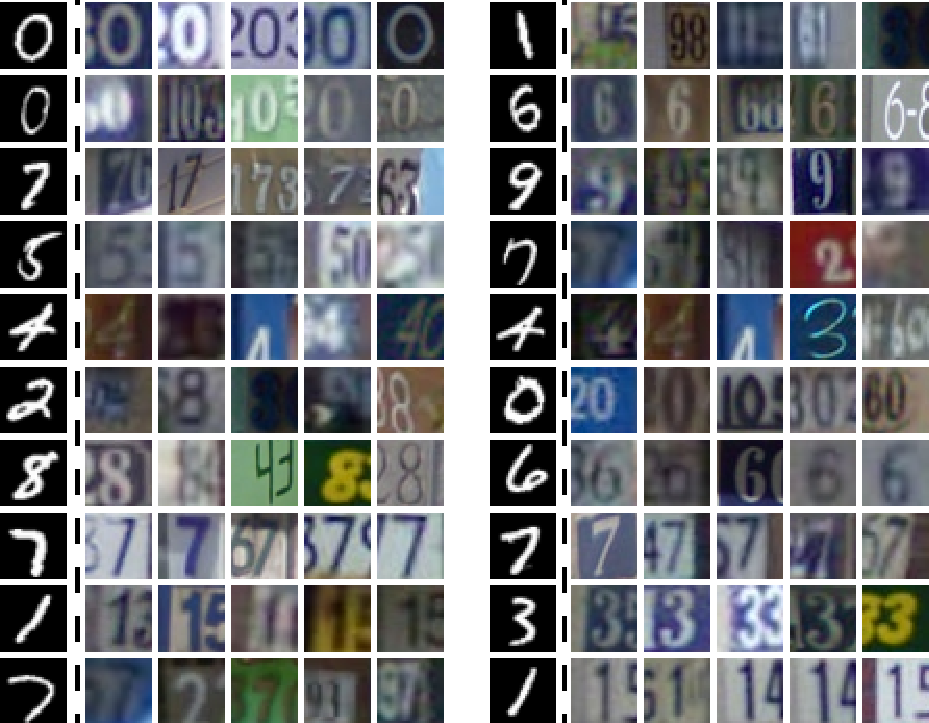
\includegraphics[width=0.4\textwidth]{nndig}
\vspace{-5mm}
\caption{Example nearest neighbors for SVHN$\rightarrow$MNIST experiment. We show an example MNIST image and 5-NN SVHN images. Please note the large domain difference.}
\label{fig:nn}
%\end{figure}
%\begin{figure}[ht]
\includegraphics[width=0.4\textwidth]{nnfi-01.png}
\caption{Example nearest neighbors for Amazon$\leftrightarrow$Webcam experiment. We show an example source image and 3-NN target images. }
%The drop in the accuracy after the nearest neighbors is expected since our loss function only models the nearest one.}
\label{fig:nnoffice}
\end{small}
\vspace{-1cm}
\end{wrapfigure}


In Figure~\ref{fig:tsnedigit}, we show the digit images of source and target after the adaptation. Clearly, the target is well clustered according to the classes and source is not very well clustered although it has some structure. Since we learn the entire network for digit classification, our networks learn discriminative features in the target domain as our loss depends directly on classification scores in target domain. Moreover, discriminative features in target arises because of the transductive modeling. In comparison, state of the art domain invariance based algorithms only try to be invariant to the domains without explicit modeling of discriminativeness on the target domain. Hence, our similarity metric explicitly models the relationship between the domains and results in an equivariant model while enforcing discriminative behavior in the target. We also draw lines between the nearest neighbor images of source and target images to show the accuracy of the metric function. Moreover, the nearest neighbors are quite accurate confirming the quantitative results. 

\subsubsection{Label propagation \& reject option}
In order to evaluate the effect of having a robust label propagation and reject option, we compare our method with self baselines. We compare our algorithm with the version neither include label propagation nor include the reject option as well as a version only include propagation. We denote them with no reject/no prop and no reject respectively. We tabulate the accuracy results from Office dataset in Table~\ref{tab:res}. Results suggests that both feature learning and reject option are crucial for successful transduction. 
%Another interesting observation is the unstable behavior when we disable label propagation. This is also expected since without label propagation, the labeling stage will have more mis-classifications and they will decrease the accuracy of the metric.
%>>>>>>> 495209cbd03d496cea6aa34df03ce5686deb5946


  
\begin{figure*}[ht]
    \begin{subfigure}[b]{0.25\textwidth}
        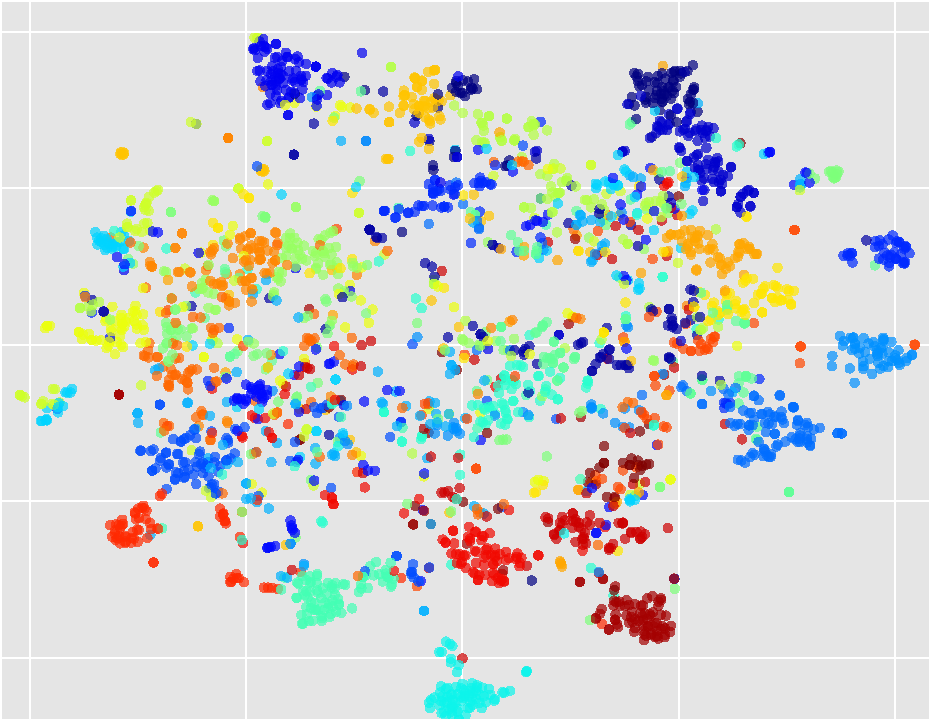
\includegraphics[width=\textwidth]{before_c_s_c}
        \caption{S. w/o Adaptation}
        \label{fig:gull}
    \end{subfigure}~\begin{subfigure}[b]{0.25\textwidth}
        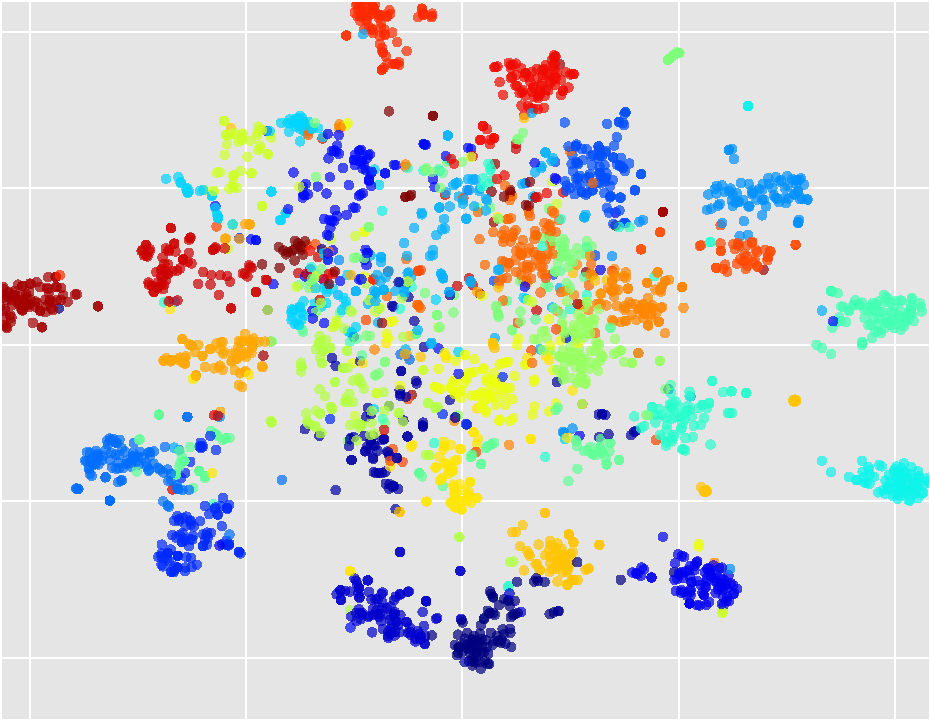
\includegraphics[width=\textwidth]{after_c_s_c}
        \caption{S. with Adaptation}
    \end{subfigure}~\begin{subfigure}[b]{0.25\textwidth}
        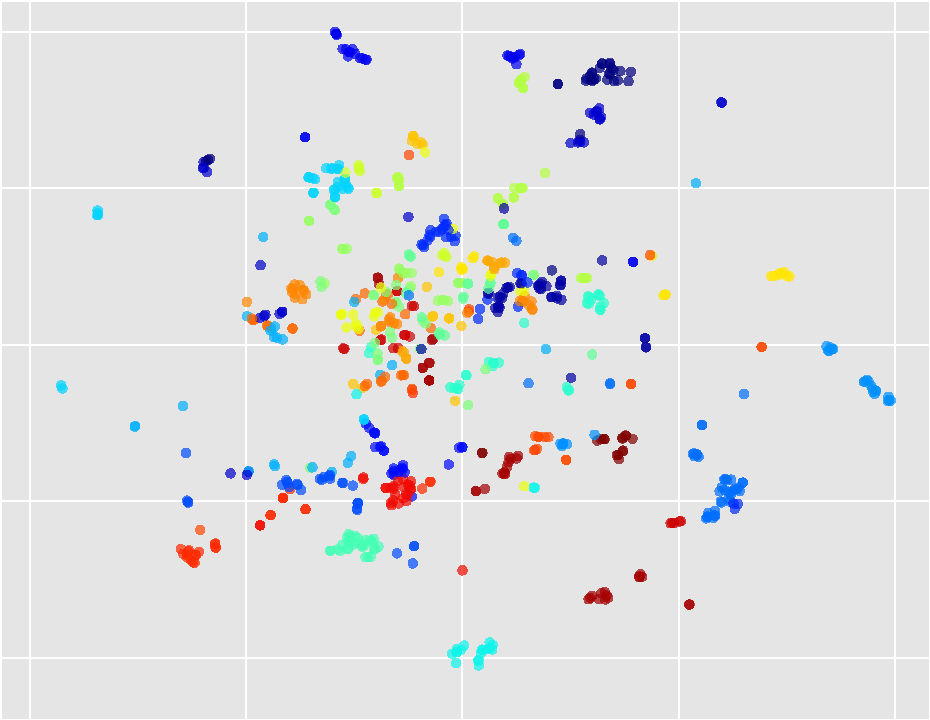
\includegraphics[width=\textwidth]{before_c_t_c}
        \caption{T w/o Adaptation}
        \label{fig:gull}
    \end{subfigure}~\begin{subfigure}[b]{0.25\textwidth}
        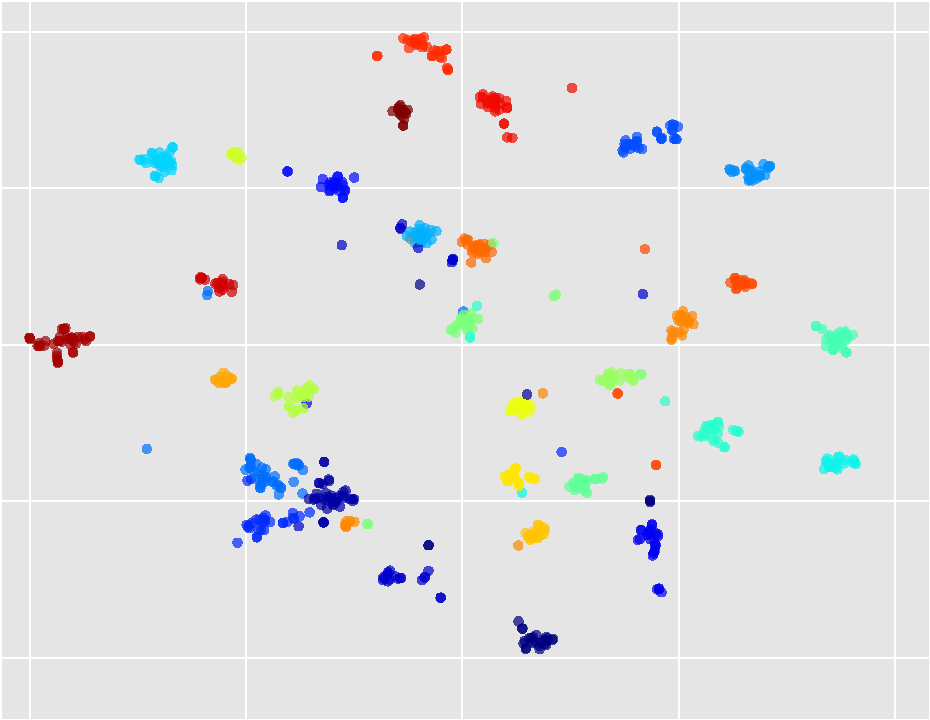
\includegraphics[width=\textwidth]{after_c_t_c}
        \caption{T with Adaptation}
    \end{subfigure}
    \caption{tSNE plots for office dataset Webcam(S)$\rightarrow$Amazon(T). Source features were discriminative and stayed discriminative as expected. On the other hand, target features became quite discriminative after the adaptation.}
    \label{fig:tsne}
        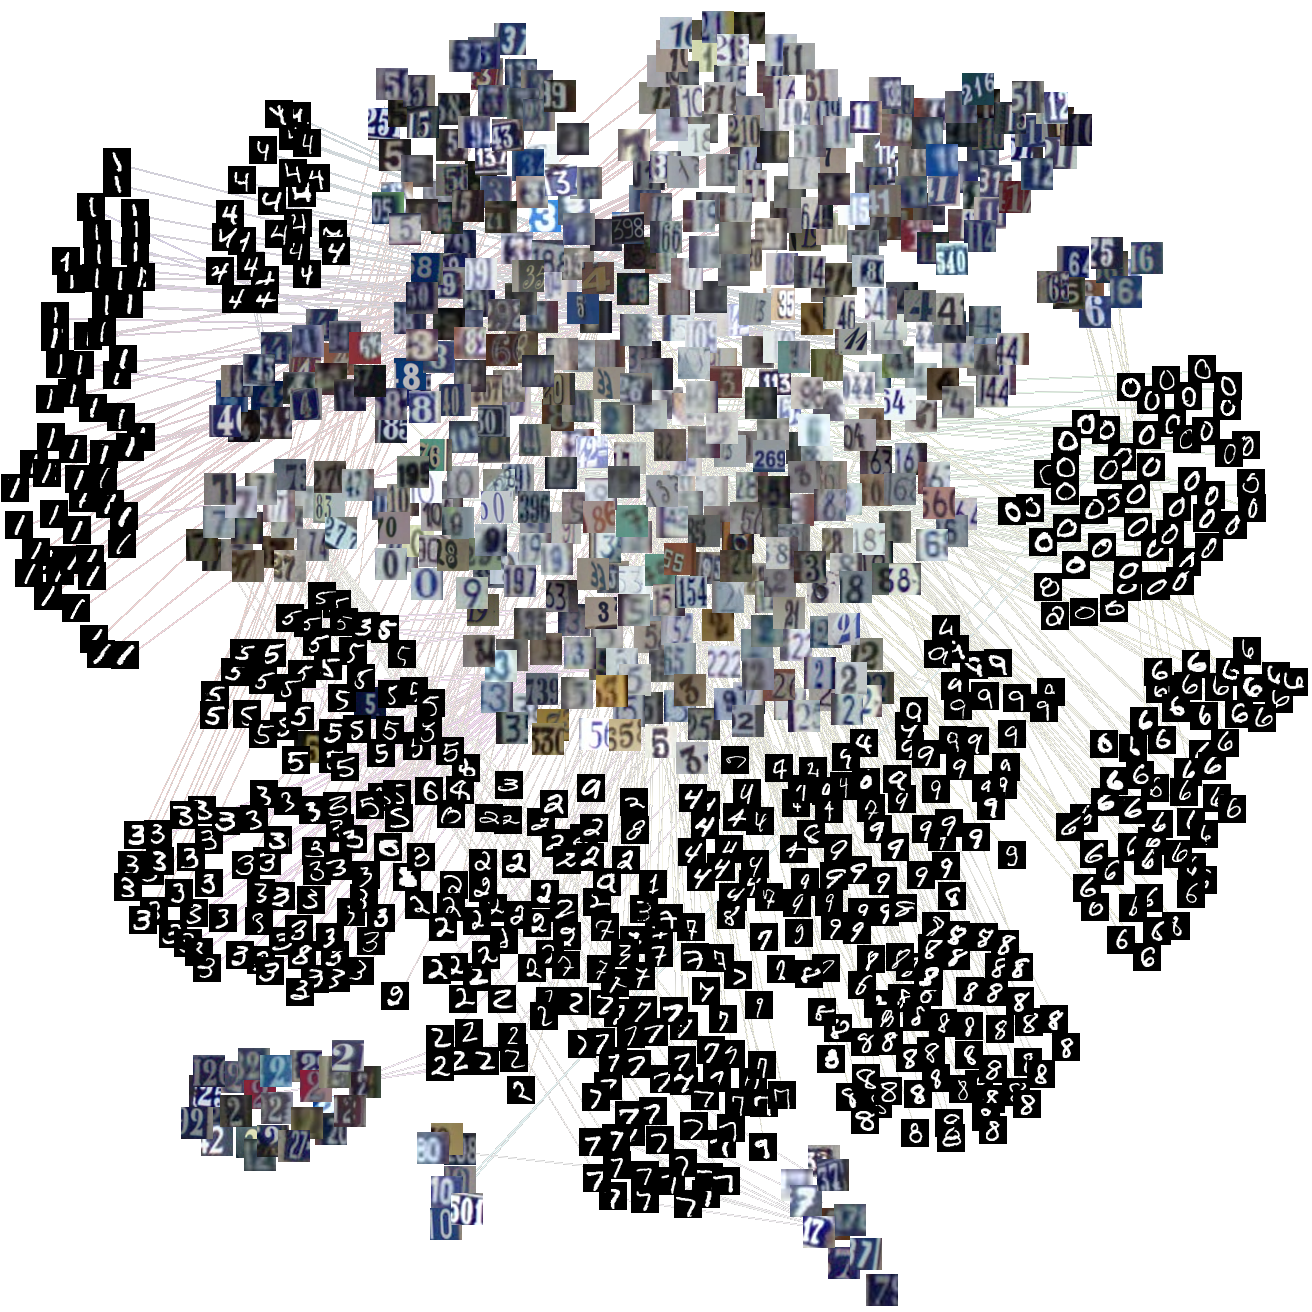
\includegraphics[width=\textwidth]{out_im.png}
        \vspace{-5mm}
\caption{tSNE plot for SVHN$\rightarrow$MNIST experiment. Please note that the discriminative behavior only emerges in the unsupervised target instead of the source domain. This explains the motivation behind modeling the problem as transduction. In other words, our algorithm is designed to be accurate and discriminative in the target domain which is the domain we are interested in.  }
\label{fig:tsnedigit}
\end{figure*}
